	
\documentclass[letterpaper, 11pt]{extarticle}
% \usepackage{fontspec}

% ==================================================

% document parameters
% \usepackage[spanish, mexico, es-lcroman]{babel}
\usepackage[english]{babel}
\usepackage[margin = 1in]{geometry}

% ==================================================

% Packages for math
\usepackage{mathrsfs}
\usepackage{amsfonts}
\usepackage{amsmath}
\usepackage{amsthm}
\usepackage{amssymb}
\usepackage{physics}
\usepackage{dsfont}
\usepackage{esint}

% ==================================================

% Packages for writing
\usepackage{enumerate}
\usepackage[shortlabels]{enumitem}
\usepackage{framed}
\usepackage{csquotes}

% ==================================================

% Miscellaneous packages
\usepackage{float}
\usepackage{tabularx}
\usepackage{xcolor}
\usepackage{multicol}
\usepackage{subcaption}
\usepackage{caption}
\captionsetup{format = hang, margin = 10pt, font = small, labelfont = bf}

% Citation
\usepackage[round, authoryear]{natbib}

% Hyperlinks setup
\usepackage{hyperref}
\definecolor{links}{rgb}{0.36,0.54,0.66}
\hypersetup{
   colorlinks = true,
    linkcolor = black,
     urlcolor = blue,
    citecolor = blue,
    filecolor = blue,
    pdfauthor = {Author},
     pdftitle = {Title},
   pdfsubject = {subject},
  pdfkeywords = {one, two},
  pdfproducer = {LaTeX},
   pdfcreator = {pdfLaTeX},
   }
\usepackage{titlesec}
\usepackage[many]{tcolorbox}

% Adjust spacing after the chapter title
% \titlespacing*{<command>}{<left>}{<before-sep>}{<after-sep>}
\titlespacing*{\chapter}{0cm}{-2.0cm}{0.50cm}
\titlespacing*{\section}{0cm}{0.50cm}{0.25cm}

% Indent 
\setlength{\parindent}{0pt}
\setlength{\parskip}{1ex}

% --- Theorems, lemma, corollary, postulate, definition ---
% \numberwithin{equation}{section}


\newtcbtheorem[]{problem}{Problem}%
    {enhanced,
    colback = black!5, %white,
    colbacktitle = black!5,
    coltitle = black,
    boxrule = 0pt,
    frame hidden,
    borderline west = {0.5mm}{0.0mm}{black},
    fonttitle = \bfseries\sffamily,
    breakable,
    before skip = 3ex,
    after skip = 3ex
}{problem}

\tcbuselibrary{skins, breakable}
%%% Commands defined by me
%   Euler constant
\newcommand{\eu}{\mathrm{e}}

%   Imaginary unit
\newcommand{\im}{\mathrm{i}}

%   Degrees
\newcommand{\grado}{\,^{\circ}}

%%% Linear Algebra

% Transpose
\newcommand{\transpose}[1]{{#1}^{\mathsf{T}}}

%%% Calculus
%   Integral from - infinity to infinity 
\newcommand{\Int}{\int\limits_{-\infty}^{\infty}}

%   Indefinite integral
\newcommand{\rint}[2]{\int{#1}\dd{#2}}

%   Definite integral
\newcommand{\Rint}[4]{\int\limits_{#1}^{#2}{#3}\dd{#4}}


% Serif bold text
\newcommand{\tsb}[1]{\textsf{\textbf{#1}}}

% Separation line
\newcommand{\linea}{\textcolor{gray!60}{\rule{\linewidth}{0.2pt}}}

% Bigger version of a \cdot to denote dot product
\makeatletter
\newcommand*\bigcdot{\mathpalette\bigcdot@{.5}}
\newcommand*\bigcdot@[2]{\mathbin{\vcenter{\hbox{\scalebox{#2}{$\m@th#1\bullet$}}}}}
\makeatother

% My Hamiltonian prefered notation
\newcommand{\Ham}{\hat{\mathcal{H}}}

%% Pre-existing commands redefined by me
% Trace of a matrix 
\renewcommand{\Tr}{\mathrm{Tr}}



\begin{document}
		\begin{Large}
		\textsf{\textbf{Cramer-Lundberg theorem}}\\
		Section 4 - Home Work 1
	\end{Large}
	
	\vspace{1ex}
	
	\textsf{\textbf{Student:}} \text{Mehrab Atighi}, \href{mailto:mehrab.atighi@gmail.com}{\texttt{mehrab.atighi@gmail.com}}\\
	\textsf{\textbf{Lecturer:}} \text{Mohammad Zokaei}, \href{mailto:Zokaei@sbu.ac.ir}{\texttt{Zokaei@sbu.ac.ir}}
	
	
	\vspace{2ex}
	
	\begin{problem}{}{problem-label}
		Proof of part b of the theorem below. \cite{Embrechts.etal1997}:
		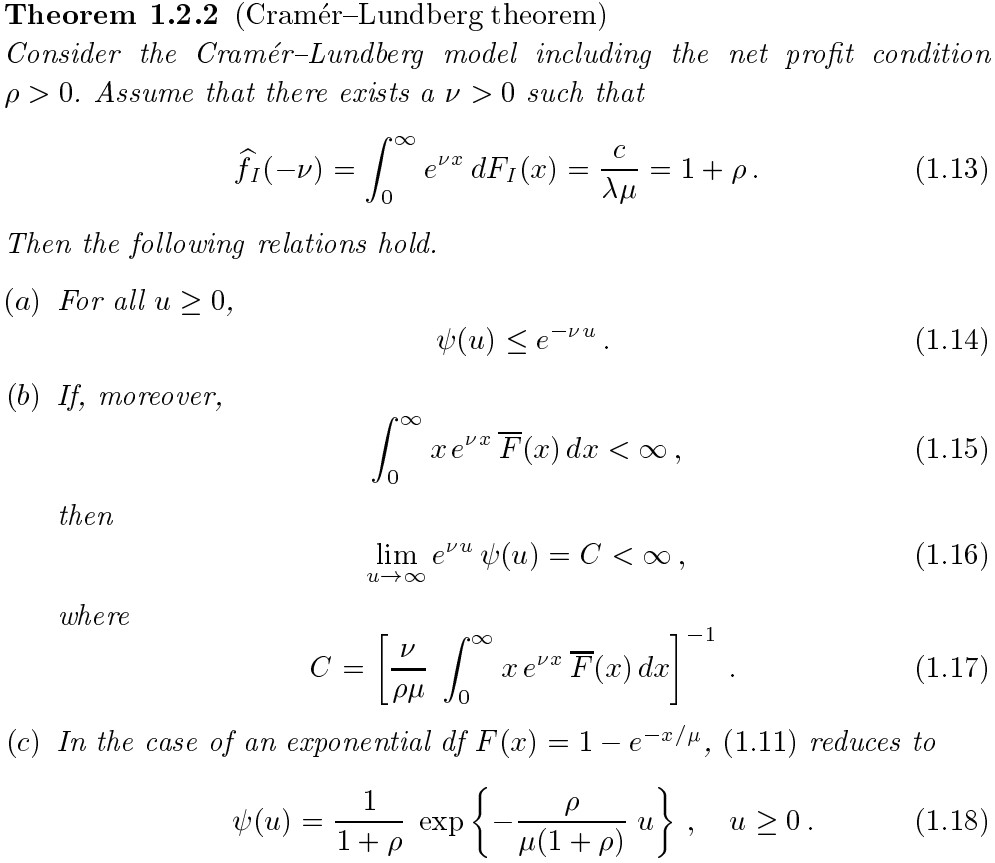
\includegraphics[width = \textwidth]{pic1.jpg}
	\end{problem}
	
	\begin{solve}{}{solve-label}
		\textbf{Proof of (b).} Denote $d(v) = -\psi'(v)$. Recall from (1.3) that $d(v)$ can be expressed via the random walk generated by $X_{i} = \xi_{i} - 1$. Then\\
		$\delta(u) = P(S(t) - ct < u \forall t > 0) \\
		= P ( \sum_{k=1}^{n} (X_k - cY_k)  \leq u \forall n \geq 1 ) $ \\
		and we now that $S(t) - ct = \sum_{k=1}^{n} (X_k -cY_k)$ so we have:\\
		$= P(\sum_{k=2}^{n} X_k - cY_k)\leq u + cY_1, - X_1  \forall n \geq 2 , X_1 - cY_1 \leq u)$ \\
		and we set $S\prime(t) = \sum_{k=2}^{n} X_k$ then we have $\sum_{k=2}^{n} (X_k -cY_k) = S\prime(t) -ct$ so we have:\\
		$= P(S'(t)-ct<u+cY_1-X_1 \forall t>0 , X_1-cY_1<u), \\
		\text{where } S' \text{ is an independent copy of } S. \text{ Hence} \\
		\delta(u)=E(P(S'(t)-ct<u+cY_1-X_1 \forall t>0 , X_1-cY_1<u|Y_1,X_1))$\\
		Considering that it was supposed to do the proof as long as we can, \textbf{I did not understand from this part onwards and I tried my best to move forward, so the effort I took to reach the next step is an image in this part}. I will add and unfortunately I could not advance the proof from here on.
		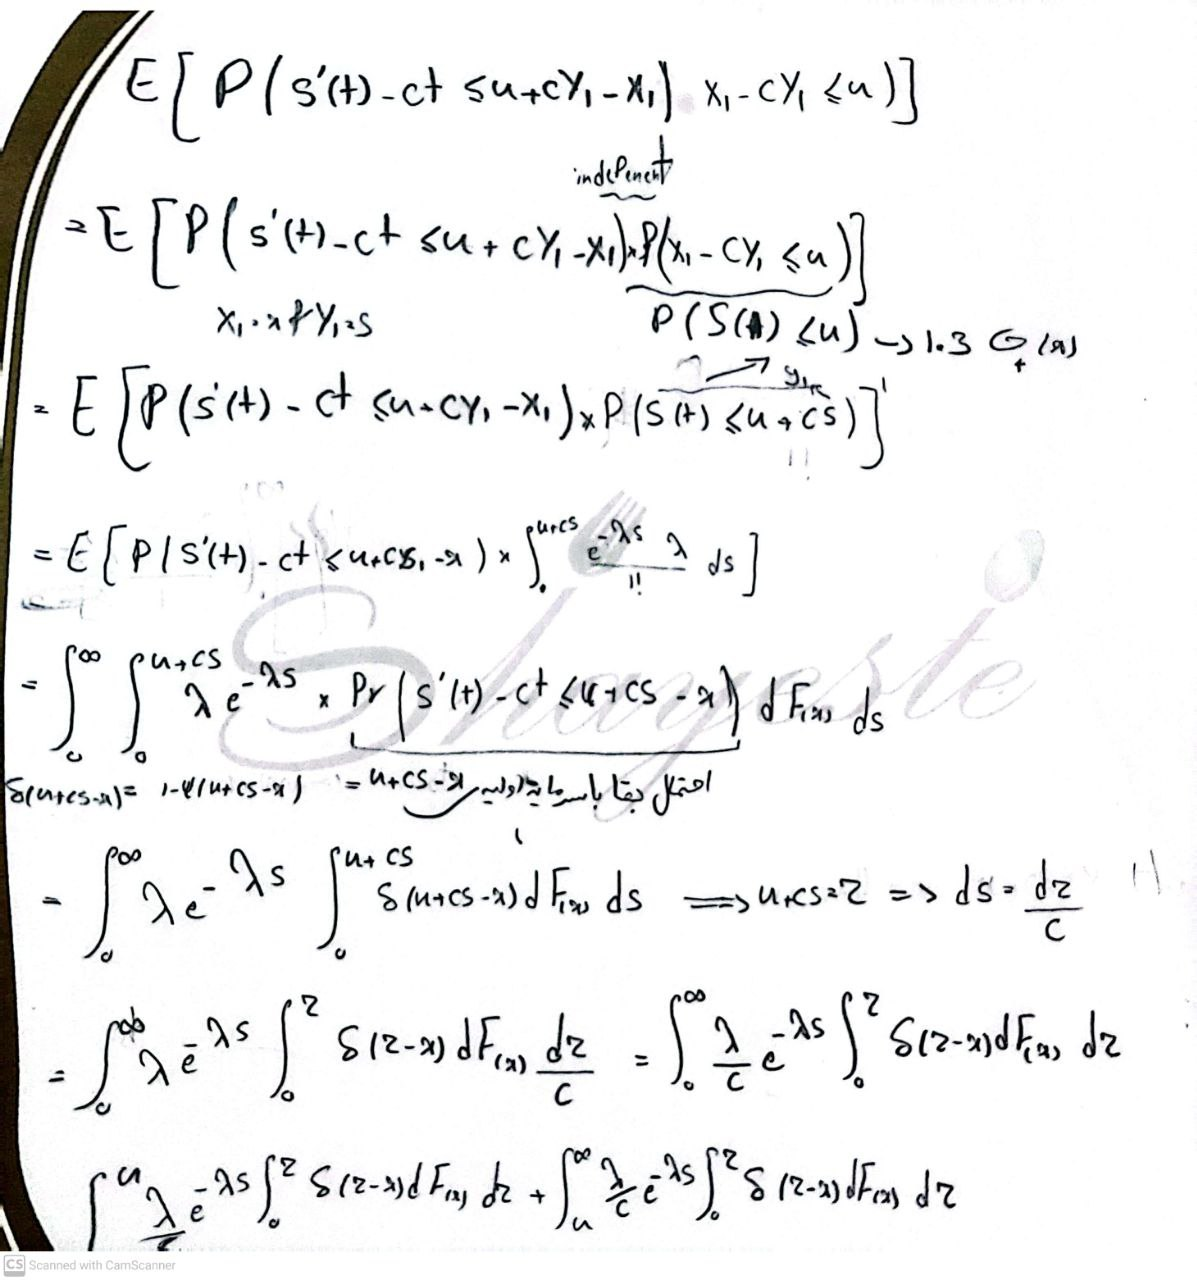
\includegraphics[width = \textwidth]{pic2.jpg}
	\end{solve}
	% =================================================
	\bibliographystyle{apalike}
	\bibliography{references}
\end{document}